\chapter{基于BLE Mesh的智能家居平台实现}
\section{开发语言的选择}
现今,市面上有许多开发语言可供选择,它们各自有各自的优点,如C/C++语言执行速度快,程序占用空间小;Go语言代码简洁,执行速度快;Dart语言易于编写,使用Flutter框架后还可实现一套代码就能编译出iOS/Android端的App。

对于本项目的BLE Mesh节点而言,其性能不高且存储空间狭小,并且需使用Nordic芯片厂商所提供的nRF5 SDK for Mesh,因此选择了C语言作为开发语言。

对于本项目的网关端而言,其性能充足但需要高扩展性且逻辑复杂,为了开发方便,因此选择了Go语言作为开发语言。

对于本项目的移动端而言,需要同时支持Android与iOS系统,为了界面逻辑统一,因此选择了Dart语言与Flutter框架作为开发语言。

\section{集成开发环境的选择}
在BLE Mesh节点开发上,目前针对嵌入式开发并支持C语言主要是SEGGER Embedded Studio及Keil,SEGGER Embedded Studio相较于Keil更加易用,并且能很好地兼容nRF5 SDK for Mesh,因此选择了SEGGER Embedded Studio作为BLE Mesh节点的集成开发环境。

在网关端开发上,目前针对Go语言的集成开发环境主要有GoLand与VS Code,但GoLand功能更为强大,能很好地进行调试以及包管理,因此选择了GoLand作为网关端的集成开发环境。

在移动端开发上,目前Google推荐使用Android Studio进行Dart+Flutter的开发,因此选择了Android Studio作为移动端的集成开发环境。

\section{逻辑部分的实现}
\subsection{BLE Mesh节点}
BLE Mesh节点主要分为两个角色,一个是Server,一个是Provisioner。Server作为连接继电器、传感器等模块的角色,而Provisioner则负责给未配置的Server节点发放BLE Mesh网络配置。

\subsubsection{Server}
Server节点在上电后初始化BLE、Mesh协议栈及其他参数,开始发送Unprovisioned Node Beacon广播信息,等待Provisioner分发配置,配网成功后注册GATT服务与传感器服务,以便移动端或网关端BLE Mesh插件通过此节点代理入网,并允许其他节点访问它的模块。

\begin{figure}[H]
    \centering
    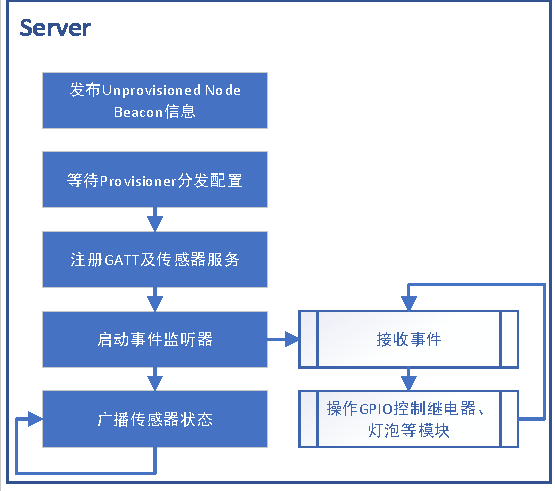
\includegraphics{flowchart_mesh_server.pdf}
    \caption{基于BLE Mesh的智能家居平台BLE Mesh Server节点流程图}
    \label{fig:flowchart_mesh_server}
\end{figure}

\begin{figure}[H]
    \centering
    \begin{lstlisting}[language=C]
        ble_stack_init();
        gap_params_init();
        conn_params_init();
        mesh_init();
        //初始化蓝牙协议栈、GATT参数、传感器参数、Mesh协议栈
        if (!m_device_provisioned){
            //设备未配网
            static const uint8_t static_auth_data[NRF_MESH_KEY_SIZE] = STATIC_AUTH_DATA;
            //配置OOB预认证密钥
            mesh_provisionee_start_params_t prov_start_params = {
                .p_static_data    = static_auth_data,
                .prov_complete_cb = provisioning_complete_cb,
                .prov_device_identification_start_cb = device_identification_start_cb,
                .prov_device_identification_stop_cb = NULL,
                .prov_abort_cb = provisioning_aborted_cb,
                .p_device_uri = EX_URI_LS_SERVER
            };
            mesh_provisionee_prov_start(&prov_start_params);
            //启动Provisionee过程,等待配网结束
        }
        mesh_app_uuid_print(nrf_mesh_configure_device_uuid_get());
        //输出配网后分配到的设备UUID以供调试使用
        mesh_stack_start();
        //启动Mesh协议栈
    \end{lstlisting}
    \caption{基于BLE Mesh的智能家居平台BLE Mesh Server节点关键代码}
    \label{fig:code_mesh_server}
\end{figure}

\subsubsection{Provisioner}

\subsection{网关端}
内容

\subsection{移动端}
内容
